\section{Use Case: Videoaufzeichnung}
\label{sec:Videoaufzeichnung}

Zunächst sollen im Folgenden die Grundlagen der digitalen Videoaufzeichnung und die dabei wichtigen Parameter erläutert werden.
Eine digitale Videoaufzeichnung besteht im Wesentlichen aus einer Folge von Bildern und eventuell einer Tonspur.
In dieser Arbeit soll der Fokus auf der visuellen Komponente liegen.
Digitalkameras, wie sie auch in Smartphones zu finden sind, verwenden zur Aufnahme der einzelnen Bilder einen oder mehrere \ac{CCD} oder \ac{CMOS} Sensoren.
Jeder Sensor besteht aus einem Raster kleiner, als Pixel bezeichnete, Sensorelemente, welche die einfallende Lichtintensität messen und diese zu einem Digitalbild kombinieren können \cite[S. 63ff.]{Szeliski_ComputerVision}.
Um Farbbilder zu gewinnen wird heute meist ein Sensor mit einer Bayer-Matrix, einem Muster aus Farbfiltern, verwendet.
So ist jeder Pixel nur für jeweils eine der Grundfarben Rot, Grün oder Blau zuständig \cite[S. 420ff.]{Schmidt_Videotechnik}.
Um ein nutzbares Bild zu erhalten, ist nach der Gewinnung der Signalpegel der einzelnen Pixel ein mehrstufiger Prozess analoger und digitaler Signalverarbeitung notwendig \cite[S. 63ff.]{Szeliski_ComputerVision}.
In \autoref{fig:ImagePipeline} ist der übliche Weg vom einfallenden Licht bis zu einem nutzbaren Digitalbild dargestellt. 
Bei der Videoaufzeichnung läuft der Prozess ähnlich ab, nur werden Bildfolgen aufgenommen und Verarbeitungen teilweise auf diesen durchgeführt.
\begin{figure}
    \centering
    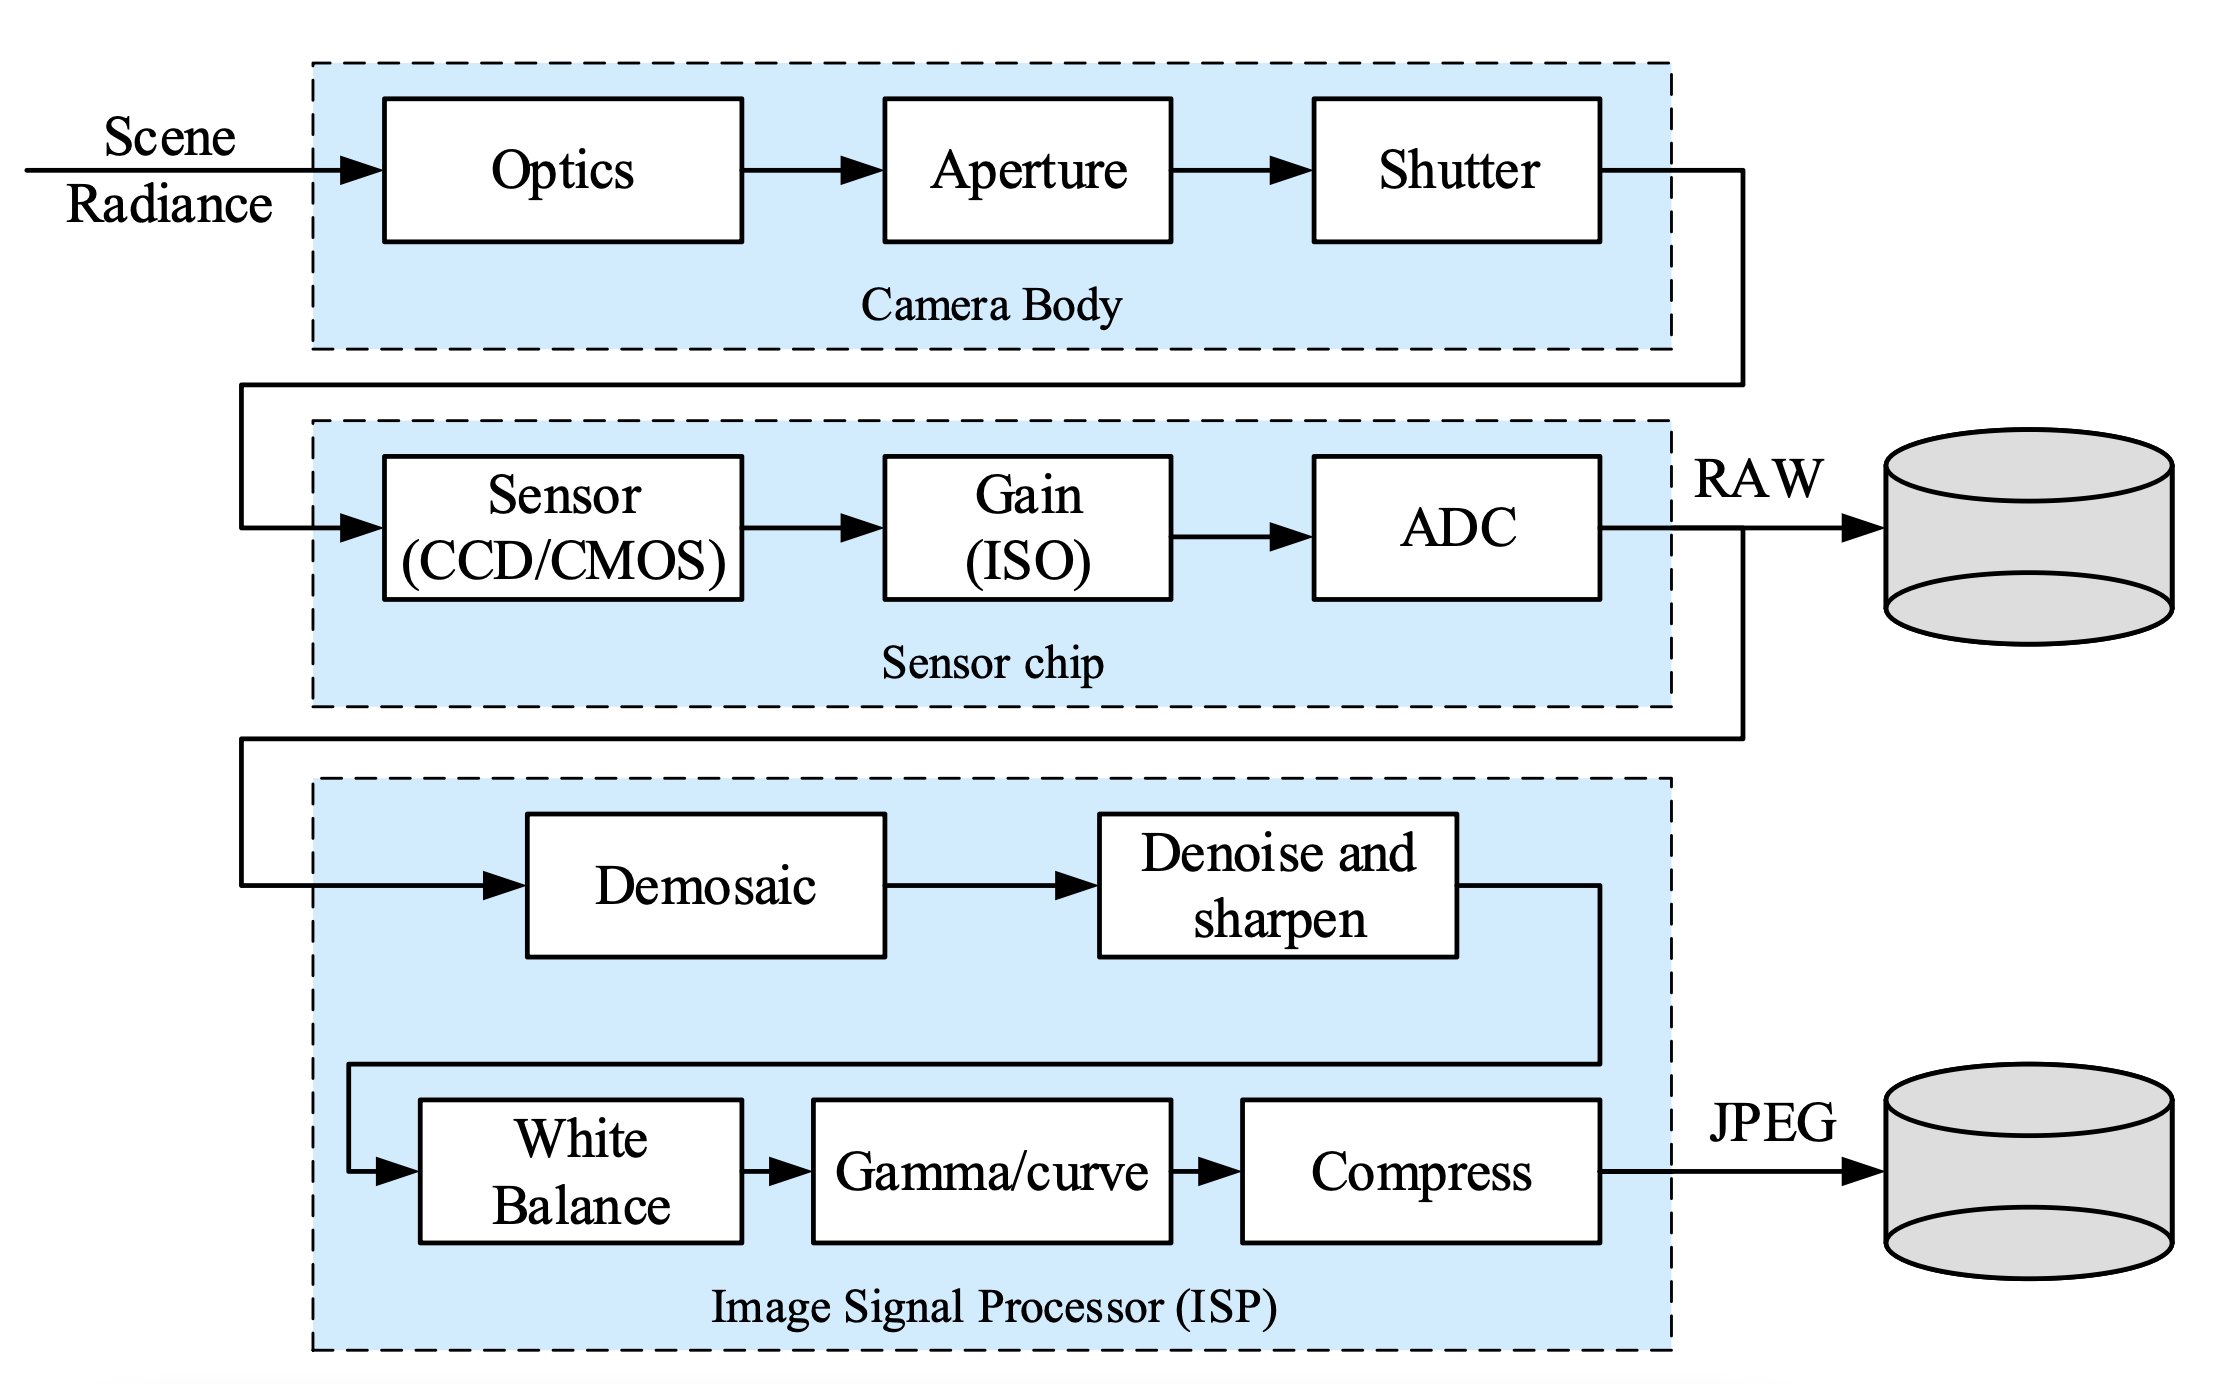
\includegraphics[width=0.85\textwidth]{ImagePipeline}
    \caption{Überblick über den Prozess der Entstehung eines Digitalbildes \cite[S. 64ff.]{Szeliski_ComputerVision}.}
    \label{fig:ImagePipeline}
\end{figure}


Das von einer digitalen Kamera aufgenommene Bild ist insbesondere von der Lichtintensität abhängig.
Diese wird vor allem durch die Belichtungszeit und die Größe der Blendenöffnung bestimmt.
Außerdem kann das Bild durch Variation der Sensorempfindlichkeit beeinflusst werden.
Die Belichtungszeit ist die Zeit, die der Sensor dem einfallenden Licht ausgesetzt ist \cite[S. 390ff.]{Schmidt_Videotechnik}.
Sensorempfindlichkeit bestimmt insbesondere die Verstärkung der elektronischen Signale und wird heute meist als \acs{ISO}-Wert, angelehnt an den zugrundeliegenden Standard der \acf{ISO}, angegeben \cite[S. 412ff.]{Schmidt_Videotechnik}.
Die Blendenöffnung ist der Durchmesser der variablen Blende, welche die Öffnung bestimmt, durch die das Licht auf den Sensor fällt \cite[S. 444ff.]{Schmidt_Videotechnik}.
Die Parameter Blendenöffnung, Belichtungszeit und Sensorempfindlichkeit werden auch als Belichtungsparameter bezeichnet.

Neben den Parametern für die Belichtung wird das Bild auch durch das verwendete Objektiv, vor allem durch Brennweite und den Fokus bestimmt.
Durch Veränderung der Brennweite lässt sich der Bildausschnitt verändern und eine Vergrößerung beziehungsweise Verkleinerung von Objekten erreichen.
Der Fokus bestimmt, welche Entfernung des Bildes scharf dargestellt wird und wird in Amateurkameras häufig automatisch eingestellt.
Die Kameras in heutigen Smartphones sind üblicherweise mit mehreren Sensoren ausgestattet, die jeweils über ein eigenes Objektiv mit unterschiedlichen Brennweiten verfügen \cite[S. 499ff.]{Schmidt_Videotechnik}.

Auch der Weißabgleich beeinflusst das Aussehen des resultierenden Bildes.
Der Weißabgleich bestimmt die Farbtemperatur des Bildes und hat die Aufgabe unabhängig von der Lichtquelle einen gleichmäßigen Farbeindruck zu erreichen.
Häufig wird der Weißabgleich automatisch eingestellt, es kann jedoch auch wünschenswert sein einen Wert vorzugeben \cite[S. 434ff.]{Schmidt_Videotechnik}.

Die wichtigsten dieser Parameter, welche bei Videoaufzeichnungen zusätzlich relevant sind, sind die Bildrate, das Kompressionsverfahren und das Bildformat.
Unabhängig vom Format und der Auflösung des Sensors bieten Kameras meist die Möglichkeit das Bildformat und damit die genutzte Fläche des Sensors und die Auflösung des resultierenden Videos zu beeinflussen \cite[S. 422]{Schmidt_Videotechnik}.
Zum Beispiel werden verschiedene Formate für verschiedene Auswertungsmedien wie Kino oder TV bevorzugt.
Die Bildrate, auch Framerate genannt, gibt an, wie viele Bilder pro Sekunde (\ac{FPS}) aufgezeichnet werden und ist damit von der Belichtungszeit abhängig.
Allgemein muss $Bildrate * Belichtungszeit \leq 1$ gelten.
Eine Bildrate von $60 fps$ mit einer Belichtungszeit von $1/30 s$ pro Bild ist beispielsweise nicht möglich, da mit dieser Belichtungszeit weniger als 60 Bilder pro Sekunde aufgenommen werden können.
Bei schnellen Bewegungen wirken bewegte Objekte in Aufnahmen mit niedriger Bildrate unscharf.
Die Bildrate wird allerdings häufig auch als kreatives Gestaltungsmittel eingesetzt \cite[S. 174f.]{Schmidt_Videotechnik}.

Bei der Wahl von Kompressionsverfahren, auch Codecs genannt, und Bitrate bei der Komprimierung spielt sowohl der verfügbare Speicherplatz als auch die gewünschte Qualität eine Rolle.
Generell gilt, dass bei niedrigerer Bitrate durch stärkere Kompression ein kleinerer Speicherbedarf auf Kosten der Qualität entsteht.
Moderne Verfahren, wie H.265 oder AV1 erreichen jedoch bei gleicher Bitrate oft eine höhere Qualität als ältere Verfahren wie H.264.
Umgekehrt kann der für die gleiche Qualität benötigte Speicherplatz reduziert werden.
Dabei ist zu beachten, dass für proprietäre Kompressionsverfahren wie H.264 oder H.265 kostenpflichtige Lizenzen benötigt werden, welche meist an die verwendete Hardware gebunden sind.
Offene Codecs, wie VP9 oder AV1, sind dagegen frei verfügbar und können auf allen Geräten verwendet werden \cite[S. 253ff.]{Schmidt_Videotechnik}.


\subsection{Für Videoaufzeichnung relevante Parameter}
\label{sec:relevante_parameter}

\autoref{tab:parameter_support} gibt einen Überblick, welche Parameter sich grundsätzlich über die \acp{API} von Android und iOS einstellen lassen.
Die Wertebereiche sind stark vom konkreten Smartphone abhängig, da es nicht nur Einschränkungen durch das Betriebssystem, sondern auch durch die Hardware geben kann.
Insbesondere proprietäre Codecs sind nicht überall in gleichem Maße verfügbar.
Ausnahmen bei der Einstellbarkeit bilden die Blende und die Brennweite, welche nur bei wenigen Android-Modellen einstellbar sind \cite{Sony_VariableZoom,VariableAperture_Smartphones}.
Ansonsten verwenden die meisten Geräte jeweils Objektive ohne variable Brennweite und Blende, sodass diese Parameter nur durch die Wahl des Objektivs angepasst werden können, da die meisten Smartphones mehrere Sensoren mit jeweils eigenem Objektiv verbauen \cite[S. 499ff.]{Schmidt_Videotechnik}.
Inwiefern die prinzipiell einstellbaren Parameter in den zu testenden Cross-Plattform Frameworks tatsächlich einstellbar sind, wird im Laufe dieser Arbeit näher untersucht.

\begin{table}[H]
    \begin{tabularx}{\textwidth}{ |l|l|X|X| }
        \hline
        \multicolumn{2}{|c|}{\textbf{Parameter}} & \textbf{Unterstützung iOS} & \textbf{Unterstützung Android}  \\
        \Xhline{0.5mm}
        \multirow{4}{*}{\parbox[c]{3mm}{\rotatebox{90}{\textbf{Belichtung}\hspace*{0.75cm}}}} & Belichtungszeit & Einstellbar \cite{iOS_VideoSettings, iOS_Exposure} & Einstellbar \cite{Android_CaptureRequest} \\
        \cline{2-4}
        & Sensorempfindlichkeit (ISO) & Einstellbar \cite{iOS_VideoSettings, iOS_Exposure} & Einstellbar \cite{Android_CaptureRequest}  \\
        \cline{2-4}
        & Blende & Nur über verschiedene Objektive & Über verschiedene Objektive \\ & & & Einzelne Modelle mit variabler Blende \cite{VariableAperture_Smartphones} \\
        \hline
        \multirow{3}{*}{\parbox[c]{3mm}{\rotatebox{90}{\textbf{Objektiv}\hspace*{0.75cm}}}} & Brennweite & Nur über verschiedene Objektive & Über verschiedene Objektive \\ & & & Einzelne Modelle mit variablem optischem Zoom \cite{Sony_VariableZoom} \\
        \cline{2-4}
        & Fokus & Einstellbar \cite{iOS_Focus} & Einstellbar \cite{Android_CaptureRequest} \\
        \hline
        & Weißabgleich & Einstellbar \cite{iOS_WhiteBalance} & Einstellbar \cite{Android_CaptureRequest} \\
        \cline{2-4}
        & Bildrate & Einstellbar \cite{iOS_Format} & Einstellbar \cite{Android_CaptureRequest} \\
        \cline{2-4}
        & Bildformat & Einstellbar \cite{iOS_Format} & Einstellbar \cite{Android_CaptureRequest} \\
        \cline{2-4}
        & Kompressionsverfahren/Codec & Einstellbar \cite{iOS_VideoSettings} & Einstellbar \cite{Android_MediaCodec} \\
        \hline
    \end{tabularx}
    \caption{Einstellbarkeit der Parameter für die Videoaufzeichnungen unter iOS und Android.}
    \label{tab:parameter_support}
\end{table}
